\documentclass[11pt]{article}
\usepackage{geometry,marginnote} % Pour passer au format A4
\geometry{hmargin=1cm, vmargin=1cm} % 

% Page et encodage
\usepackage[T1]{fontenc} % Use 8-bit encoding that has 256 glyphs
\usepackage[english,french]{babel} % Français et anglais
\usepackage[utf8]{inputenc} 

\usepackage{lmodern,numprint}
\setlength\parindent{0pt}

% Graphiques
\usepackage{graphicx,float,grffile,units}
\usepackage{tikz,pst-eucl,pst-plot,pstricks,pst-node,pstricks-add,pst-fun,pgfplots} 

% Maths et divers
\usepackage{amsmath,amsfonts,amssymb,amsthm,verbatim}
\usepackage{multicol,enumitem,url,eurosym,gensymb,tabularx}

\DeclareUnicodeCharacter{20AC}{\euro}



% Sections
\usepackage{sectsty} % Allows customizing section commands
\allsectionsfont{\centering \normalfont\scshape}

% Tête et pied de page
\usepackage{fancyhdr} \pagestyle{fancyplain} \fancyhead{} \fancyfoot{}

\renewcommand{\headrulewidth}{0pt} % Remove header underlines
\renewcommand{\footrulewidth}{0pt} % Remove footer underlines

\newcommand{\horrule}[1]{\rule{\linewidth}{#1}} % Create horizontal rule command with 1 argument of height

\newcommand{\Pointilles}[1][3]{%
  \multido{}{#1}{\makebox[\linewidth]{\dotfill}\\[\parskip]
}}

\newtheorem{Definition}{Définition}

\usepackage{siunitx}
\sisetup{
    detect-all,
    output-decimal-marker={,},
    group-minimum-digits = 3,
    group-separator={~},
    number-unit-separator={~},
    inter-unit-product={~}
}

\setlength{\columnseprule}{1pt}

\begin{document}

\textbf{Nom, Prénom :} \hspace{8cm} \textbf{Classe :} \hspace{3cm} \textbf{Date :}\\

\begin{center}
  \textit{Si nous faisions tout ce dont nous sommes capables, nous nous surprendrions vraiment.}  - \textbf{Thomas Edison}
\end{center}

\subsubsection*{Cours}

\begin{itemize}
  \item \textbf{Angle droit : } \dotfill
  \item \textbf{Angle plat : } \dotfill
  \item \textbf{Angles complémentaires : } \dotfill
  \item \textbf{Angles supplémentaires : } \dotfill
\end{itemize}

\subsubsection*{Ex1 : Calculer}

\begin{figure}[H]
  \centering
  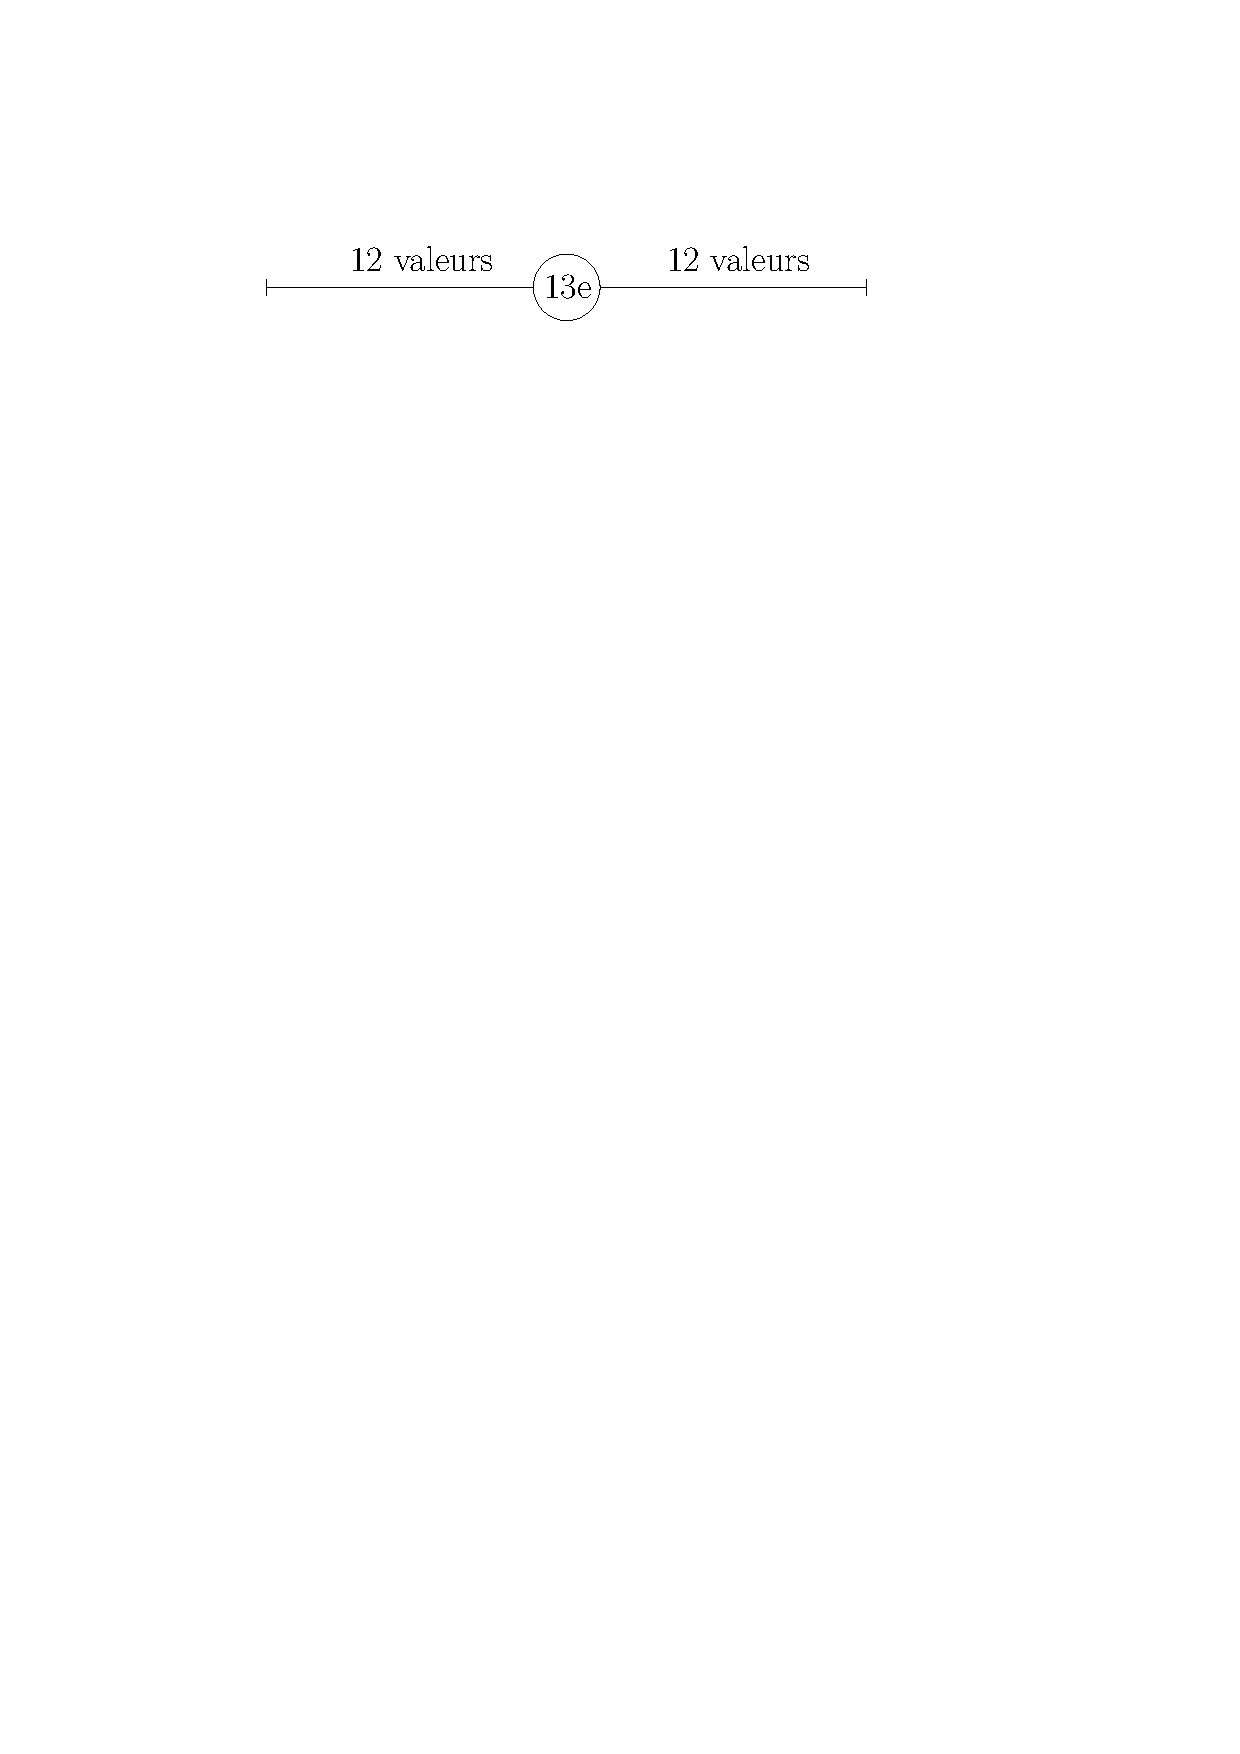
\includegraphics[width=0.8\linewidth]{5x8-angles/ex1.pdf}
\end{figure}

\begin{multicols}{5}
\begin{itemize}
  \item \dotfill
  \item \dotfill
  \item \dotfill
  \item \dotfill
  \item \dotfill
\end{itemize}
\end{multicols}

\subsubsection*{Ex2 : Calculer}

\begin{figure}[H]
  \centering
  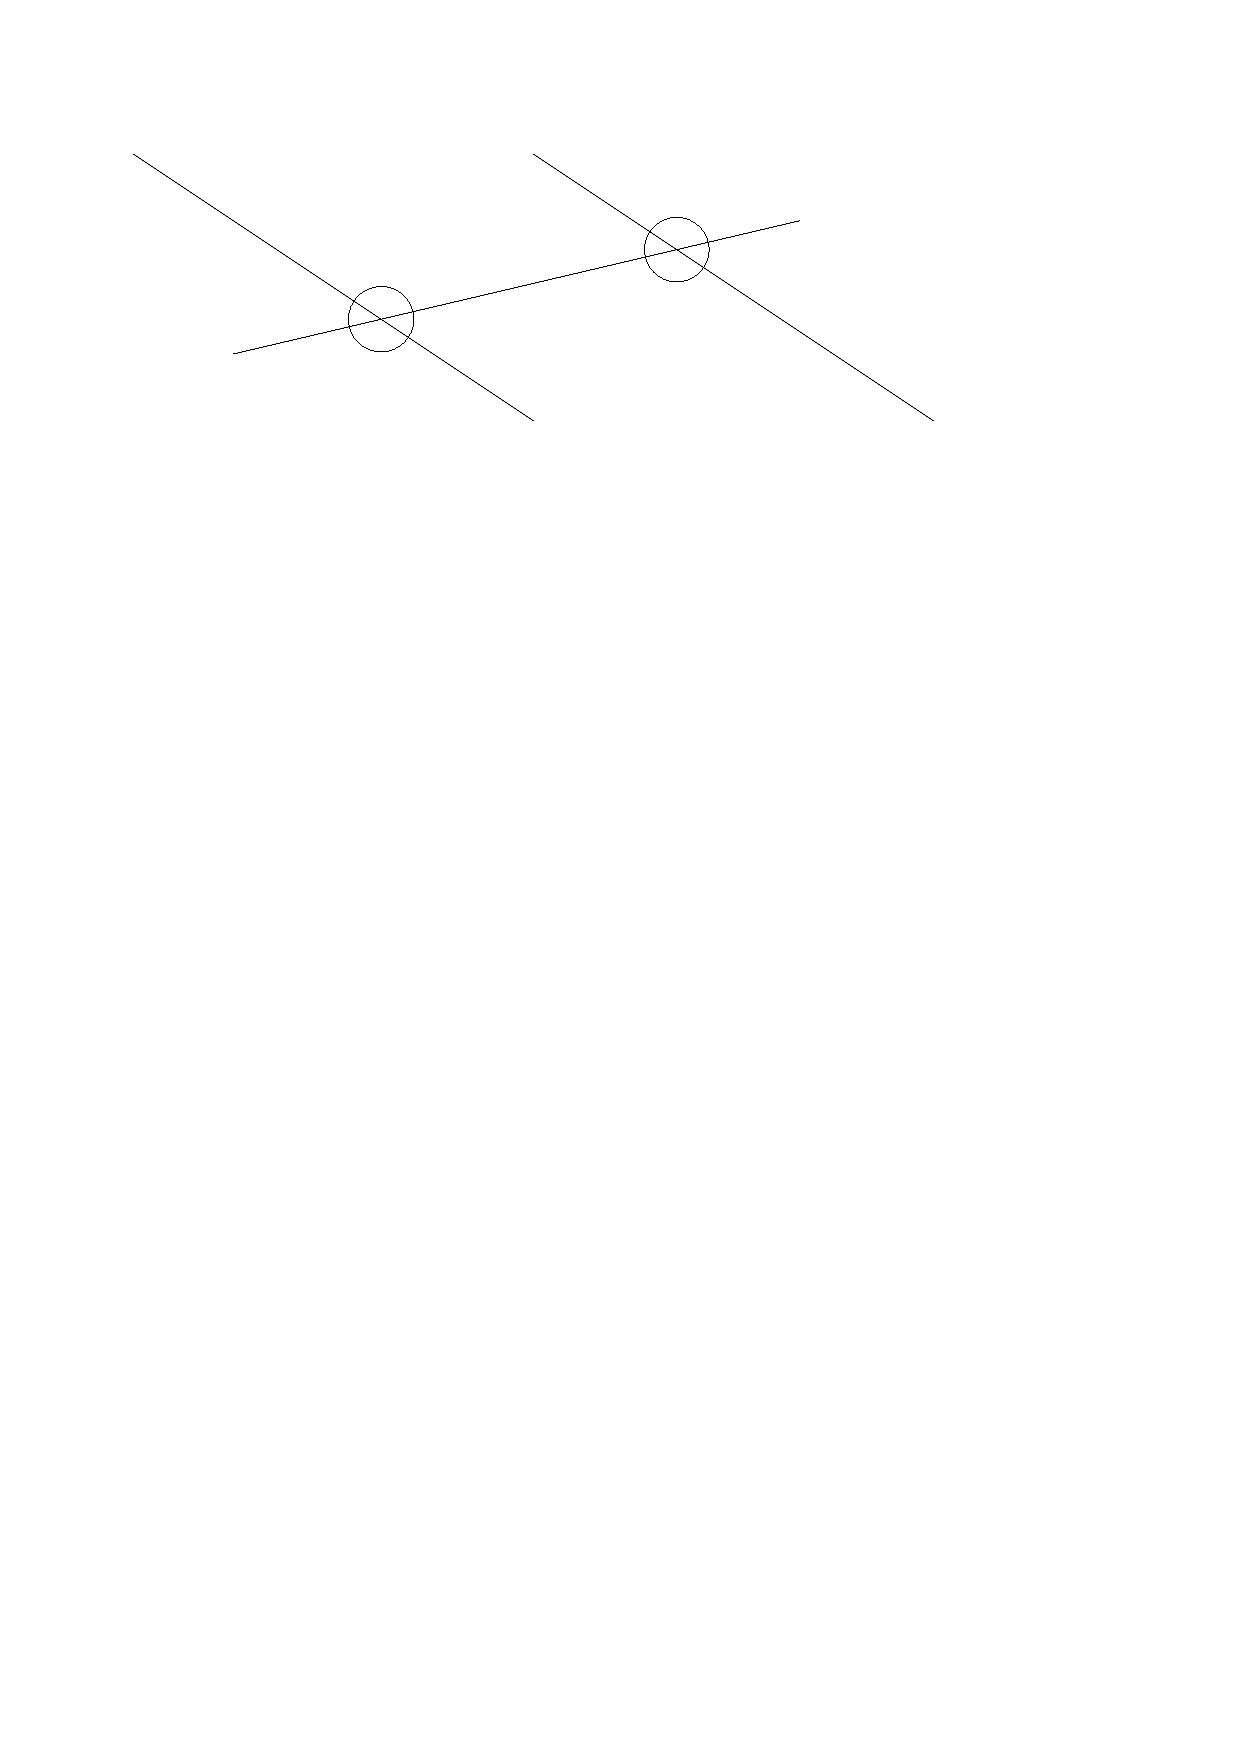
\includegraphics[width=0.6\linewidth]{5x8-angles/ex2a.pdf}
\end{figure}

\subsubsection*{Ex3 : Compléter}

\begin{figure}[H]
  \centering
  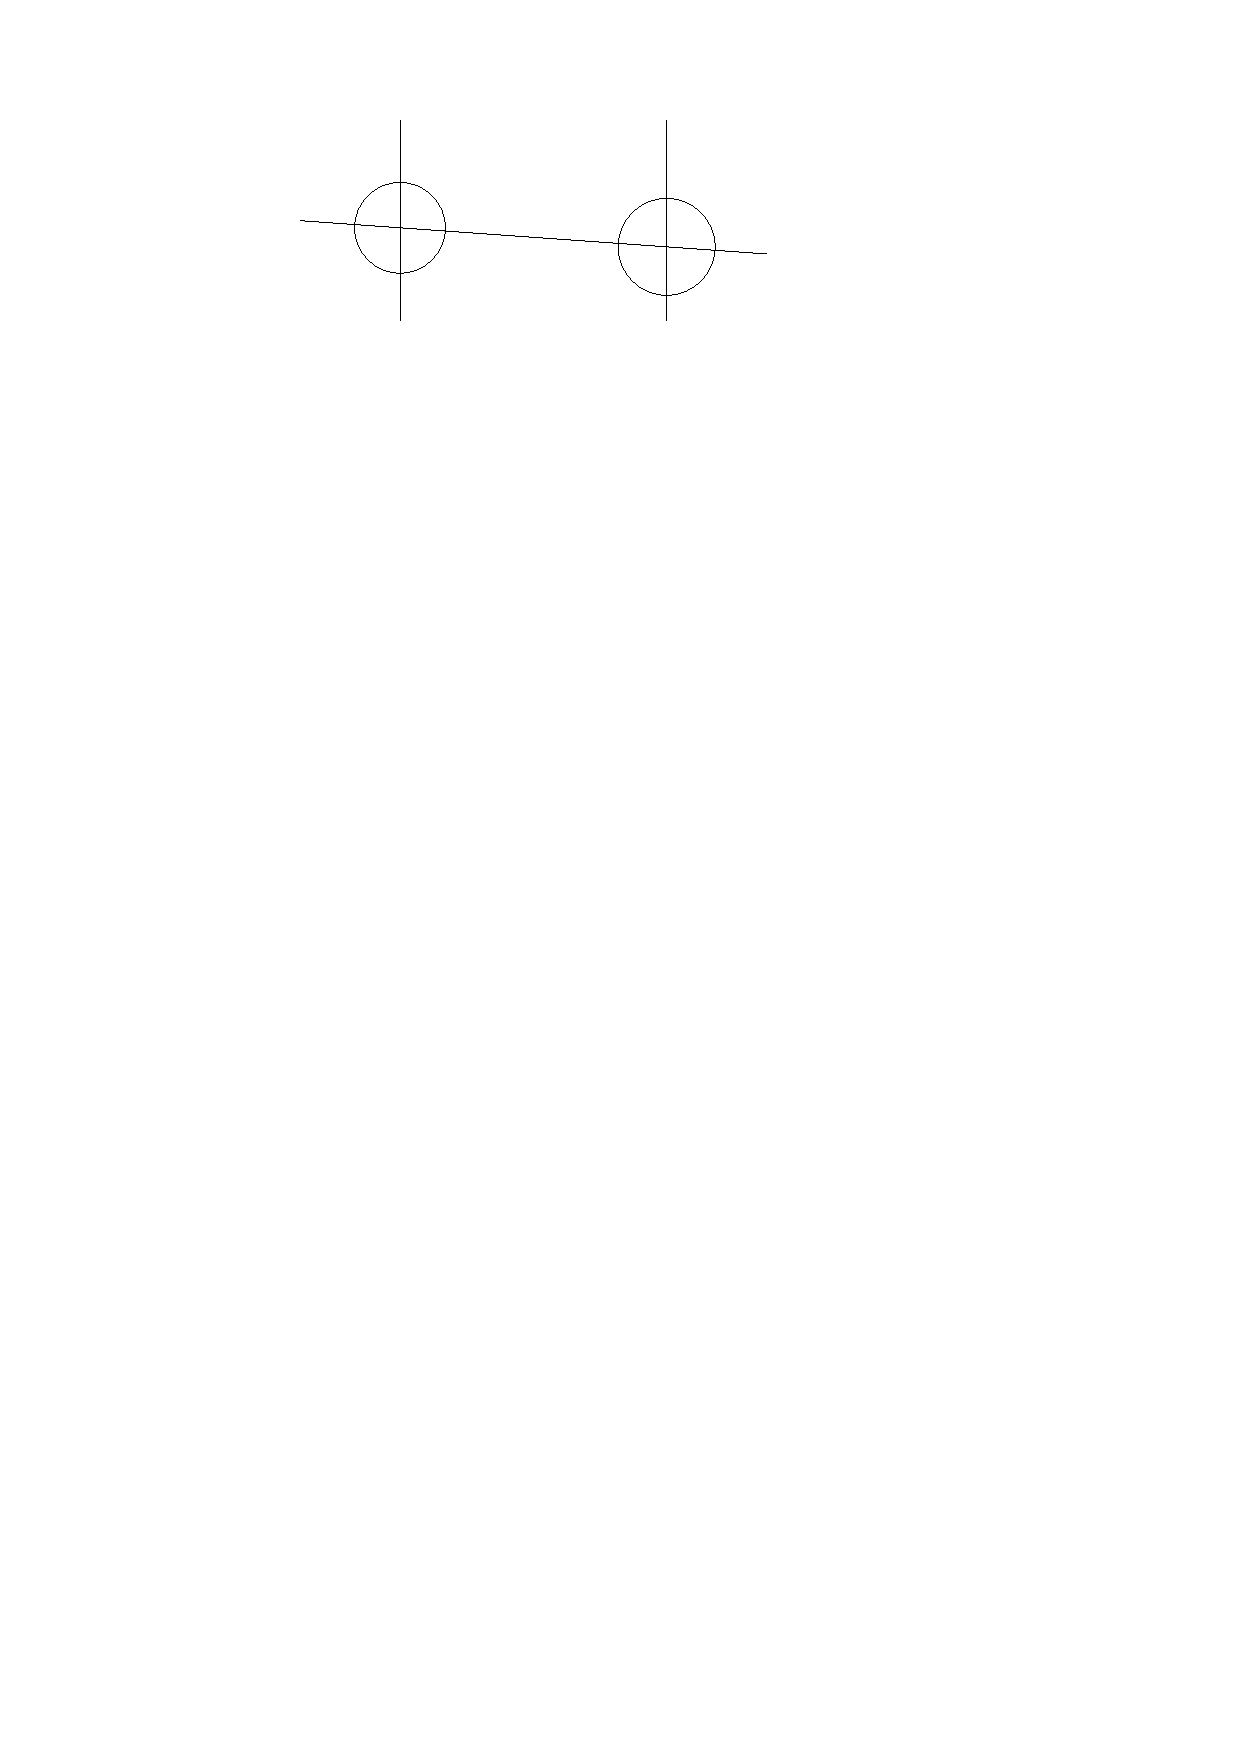
\includegraphics[width=0.5\linewidth]{5x8-angles/ex3.pdf}
\end{figure}


\begin{itemize}
  \item Les angles \hspace{1cm} et \hspace{1cm} sont : \dotfill
  \item Les angles \hspace{1cm} et \hspace{1cm} sont : \dotfill
  \item Les angles \hspace{1cm} et \hspace{1cm} sont : \dotfill
  \item Les angles \hspace{1cm} et \hspace{1cm} sont : \dotfill
  \item Les angles \hspace{1cm} et \hspace{1cm} sont : \dotfill
  \item Les angles \hspace{1cm} et \hspace{1cm} sont : \dotfill
  \item Les angles \hspace{1cm} et \hspace{1cm} sont : \dotfill
  \item Les angles \hspace{1cm} et \hspace{1cm} sont : \dotfill
\end{itemize}



\end{document}